\textbf{NOTE:} A recording of this procedure can be viewed on Asciinema at the following link: \url{https://asciinema.org/a/x8wRWlMvEh5Y8aBImklUvLzYZ}
\begin{enumerate}
    \item Step-by-Step Procedure:
        \begin{enumerate}
            \item Set up a Cloudlab instance with the default Hadoop configuration (by \lstinline{gary}).
            \item Have SSH RSA keys setup so you can copy to the Cloudlab instance.
            \item On your local machine, open up terminal and go to the directory that contains \lstinline{copy.sh} from this project.
            \item Run \lstinline{./copy.sh}. It takes 2 arguments:
                \begin{itemize}
                    \item \lstinline{username@address}. This is your username and Hadoop cluster address.
                    \item Path to private RSA key. This is used to authenticate you to use scp.
                \end{itemize}
            \item SSH into the Hadoop Cluster. The copy script from Step (d) created a directory in your home directory called \lstinline{mapreduce}, which has everything.
            \item Go into \lstinline{~/mapreduce}. To simply run Hadoop on files, run the following: \begin{verbatim}./execute.sh data/100-0.txt data/test.txt\end{verbatim} It automates the entire procedure of copying files over to HDFS and doing the Mapreduce for you.
            \item The \lstinline{py/query.py} script will run automatically after completion. Type in a few words!
            \item After the script's completion, you will see a \lstinline{results.txt} file created in the local directory. To run the query script on this file, run the following: \begin{verbatim}python3 py/query.py results.txt\end{verbatim}
           \end{enumerate}
    \item Screenshots of commands running: \\
    
\begin{figure}[!htbp] 
 \frame{ 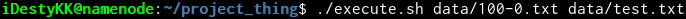
\includegraphics[width=\textwidth]{hadoop_run.png}}
  \caption{An example of the run script.}
\end{figure}

\end{enumerate}